% NOTE - this is only a template without real arguments
\begin{entry}{Phase 3 completion}{Dec 31, 2021}
    \objective 
    
    Complete, test, and refactor phase 3. (Note: completed well before this date, just updating the journal)


    \outline

    \begin{itemize}
        \item Establish RWHDERS class
        \item Write RWHDERS method to access emulator data
        \item Write RWHDERS assignment method
        \item Test RWHDERS assignment
        \item Write RWHDERS processing method
        \item Test RWHDERS processing to output
        \item Functional test MC: Emulator changes - RWHDERS input - states output - Conversion - Input - Sim - Output - Logs
    \end{itemize}

    \procedures

    \section*{Establish RWHDERS class}
    RWHDERS is the second DER-S class implemented, so it is the first case in which DER-S standardization is used. DER-S
    standardization is a function of the output of the class, since the DER-S concept allows for a wide array of inputs,
    processing functionality, etc. The following are the required components of any DER-S class:
    \begin{itemize}
        \item Attribute \verb|self.der_em_input_request|: this attribute contains the data required each time step to
            update DER-EMs with the most current data from the DER-S. It is a list of dictionarie, with key-value pairs
            containing {DER_Name:Power_in_W} data for each DER handled by the DER-S.
        \item Method \verb|self.initialize_der_s(self)|: Initializes the DER-S by reading files, connecting to emulators,
            etc. Called during the MC simulation startup process, and generally speaking, generates some attribute or
            dictionary containing the names of each DER and their respective locational data for assignment to DER-EMs.
        \item Method \verb|self.assign_der_s_to_der_em(self)|: Called by the DER assignment handler object for each
            active DER-S. Uses data from within the DER-S to assign DER-EMs to DERs at the proper topological locations.
        \item Method \verb|self.get_input_request(self)|: Returns the \verb|self.der_em_input_request|. Generally, will
            also call a DER-S function to update the input request. Called each timestep by the timekeeper to transfer
            input request data from the DER-S to the Input Handler to be updated into the EDM.
    \end{itemize}
    Further attributes or methods are not standardized between DER-Ss and will make up the "processing" functionality
    which turns input data to the DER-S into the DER-EM Input Request format for the class (either by parsing it directly
    or possibly even having to calculate it based on input parameters, label plate data, etc.)

    \section*{Write RWHDERS method to access emulator data}
    \verb|rwhders.initialize_der_s():| calls \verb|rwhders.parse_input_file_names_for_assignment()|. The method we've
    chosen to use for RWHDERS is to circumvent communications protocol requirements by having the emulators write
    DER input data to text files, which are formatted with the proper identification, location, and power data. So, to
    access emulator data, RWHDERS must read these files. The input file names contain both the DER name and location, so
    a string parser seperates out that data for use by assignment and the identification dictionary (which keeps the\
    internal DER names associated with the file names for each without requiring parsing every time step.)

    \subsubsection*{Write RWHDERS assignment method}
    Since the file parsing method has already created an input identification dictionary, this assignment method is
    routine. It grabs each line of the dictionary (containing the DER name and location), then via the assignment handler
    associates each name with the mRID of a DER-EM on the proper bus.

    \subsubsection*{Test RWHDERS assignment}
    Not fully completed. Testing RWHDERS assignment requires the emulator output files to be generated, and the GSP isn't
    quite there yet. Mock input files work fine, however.

    \subsubsection*{Write RWHDERS processing method}
    This turned out to be extremely simple, since the input files contain direct power values. It just needs to read the
    power from the files and update the input request dictionary once per time step. If the emulators were to instead
    provide "exporting/importing" flags and label plate data, as was expected, the der-em input request method would
    need to be updated to calculate power based on operating parameters.


    \section*{Testing}
    As mentioned, testing is being pushed off until the GSP is more complete. A lot of the test plan tests require more
    sophisticated inputs than can be generated in mockups. For instance: the input files for RWHDERS are static. Since
    they can't be modified during the simulation, their values are unchanging, and therefore changes can't be tested
    during the simulation or seen in the outputs. We tested as much as we could and everything seems to be working as
    intended, but this won't be confirmed until the system is gearing up for actual testing.

    \parameters
    
    N/A

    \observations

    RWHDERS turned out to be simple since we made some comprimises with the GSP team to simplify interactivity. Both
    systems can easily generate, read, or parse text files, and the nature of the data is so simple that it makes sense
    to just come up with a scheme for ourselves. This does limit the ME to a new requirement: it must be run on the
    same system as the GSP program; though, we were largely expecting that anyways and there's not a compelling reason
    to run them on seperate systems in the first place.


    \data

    Most of the relevent data can be found in the logs. The RWHDERS input files are (and must be) located in the
    "RWHDERS Inputs" directory in the ME folder, as seen on the GitHub.

    The individual dictionaries communicated from actor to actor are manipulated using complex and often repetitious
    methods. To see the contents of a dictionary at a given simulation time, the best way to go about it is to add
    a print() function to the code and read it in the terminal.

    \results
    
    RWHDERS complete. Partial functional testing completed sat, full testing pending completion of GSP.


\end{entry}


%\begin{entry}{CMake Error running EGOT-DCM Dockerfile}{Dec 02, 2020}
%    \objective
%
%    Determine the cause of the CMake error while running the dockerfile and modify file to get it to successfully build.
%
%    \outline
%
%    \begin{itemize}
%        \item Try running to see if it was just Lorry or a machine issue.
%        \item If it is a machine issue, modify configurations to ensure interoperability.
%        \item If I get the error track down its cause and modify dockerfile to fix.
%        \item Repeat until all builds are successful.
%    \end{itemize}
%
%    \procedures
%
%    \begin{itemize}
%        \item \mint{console}|git clone https://github.com/EGoT-DCS-SunSpec-Modbus|
%        \item \mint{console}|docker build -f Dockerfile.buster -t egot-dcs .|
%        \item \mint{console}|docker container run -i egot-dcs|
%    \end{itemize}
%
%    \observations
%
%    \begin{error}{Cmake Error: No CMAKE\_CXX\_COMPILER found}
%        \begin{figure}[H]
%            \centering
%            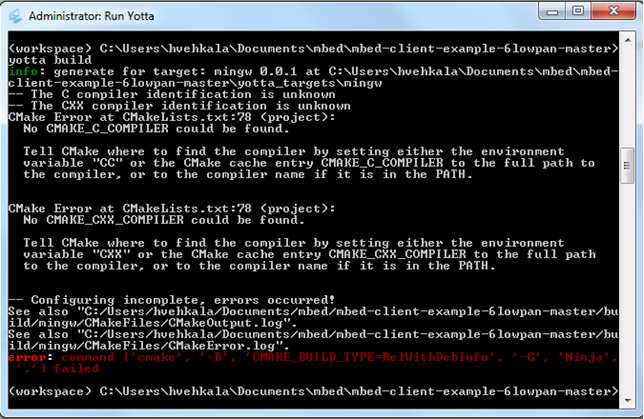
\includegraphics[height=4in]{Fall2020/Figures/cmake_error.png}
%        \end{figure}
%
%        Solution: what you need to do found at \cite{CMAKE-Forum}
%    \end{error}
%
%    \results
%
%    Short: No.
%
%    Long: Well...
%
%
%\end{entry}